% !TeX spellcheck = en_US
% !TeX root = ../main.tex
\section{Data}
\label{sec:data}

In this section, we introduce our network model of legal documents (\ref{subsec:data:model}) and instantiate it for our original dataset (\ref{subsec:data:instance}).

\vspace*{6pt}
\subsection{Data Model Specification}\label{subsec:data:model}

As visualized in Figure~\ref{fig:legal-system}~(a), the legal system consists of multiple levels: 
the local (e.g., municipal) level, the intermediate (e.g., state or province) level, the national (e.g., federal) level, and the supranational (including international) level.
Horizontally, it is usually subdivided into the legislative, executive, and judicial branches of government. 
These public parts are framed by the private sector, which operates on all levels, and the research community, which studies all parts of the legal system (including itself \cite{katz2011,newton2011,schwartz2011,george2006,ellickson2000}).
In all parts of the legal system, agents of varying sizes produce different types of outputs that create, modify, delete, apply, debate, or evaluate legal rules.
These agents and their typical outputs are summarized in Table~\ref{tab:legal-system}.

\begin{figure}
    \centering
    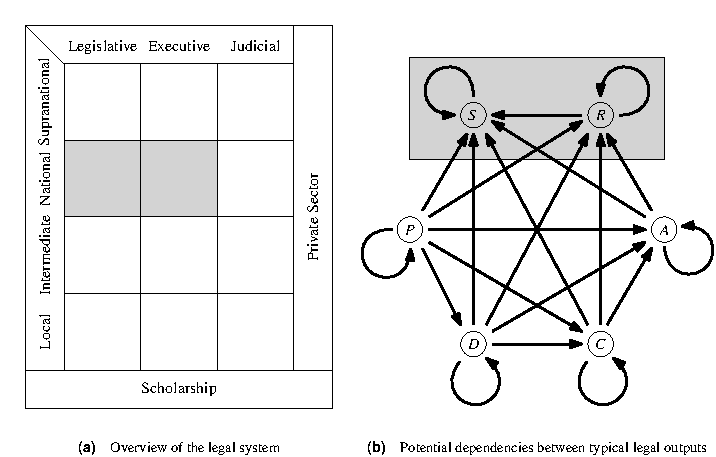
\includegraphics[width=\textwidth]{figure_1}
    \caption{Two-dimensional overview of the legal system (left) and dependencies between its typical outputs (right), with the areas covered by the dataset introduced in this work highlighted in grey. 
    The legal outputs in Panel~(b) are (clockwise from the top left and in reverse topological order) \textbf{S}tatutes, \textbf{R}egulations, Administrative \textbf{A}cts, \textbf{C}ontracts, (Court) \textbf{D}ecisions, and (Scholarly) \textbf{P}ublications.
    The arrows illustrate typical dependencies between the document types, e.g., through explicit references from arrow tails to arrow heads (although in reality, most dependencies can be bidirectional, e.g., some courts also cite legal scholarship). 
    Note that the sources covered by our dataset lie at the end of all typical dependency chains (i.e., statutes and regulations are last in the topological order of the dependency graph).
    }\label{fig:legal-system}
\end{figure}

 \begin{table}
	\centering
	\renewcommand{\arraystretch}{1.5}
\small
    \begin{tabular}{rllllll}
		\toprule&\multicolumn{3}{c}{\bfseries Branch of Government}&\bfseries Private Sector&&\bfseries Scholarship\\
		&\bfseries Legislative & \bfseries Executive & \bfseries Judicial&&&\\\midrule
		\bfseries Typical Large Agent&Parliament&Agency&Court&Firm&&Institute\\
		\bfseries Typical Small Agent&Parliamentarian&Bureaucrat&Judge&Individual&&Scholar\\
		\bfseries Typical Output(s)&Statute&Regulation&Decision&Contract&&Publication\\[-6pt]
		&&Administrative Act&&\\
		\bottomrule
	\end{tabular}

	\caption{Overview of agents and outputs in the legal system.}\label{tab:legal-system}
\end{table}

As the agents interact, they consciously interconnect their outputs. 
For example, court decisions regularly contain references to statutes, regulations, contracts, and other court decisions.
Figure~\ref{fig:legal-system}~(b) gives an overview of the classic dependencies between the typical outputs of agents in the legal system.
It illustrates that the \emph{documented} part of the legal system constitutes a multilayered document network, 
which is changing over time as the agents continue producing or amending their outputs.
Since the connections between the legal documents are placed deliberately by the agents, they encode valuable information about the content and the context of these documents. 
A lot of this information cannot be inferred from the documents' language alone (reliably or at all).
Therefore, investigating the dynamic document network representation of a legal system using network analytical tools promises insights into its structure and evolution that would be hard or impossible to obtain via other methods. 

To perform network analysis of a dynamic network of legal documents, we need to represent it as a series of graphs. 
Here, we build on a generalizable network model of statutory materials \cite{katz2020} and exploit the fact that the typical outputs listed in Table~\ref{tab:legal-system} have three common features (beyond the obvious characteristic that they all contain \emph{text}):
\begin{enumerate}
    \item They are hierarchically structured (\emph{hierarchy}).
    \item Their text is placed in containers that are sequentially ordered and can be sequentially labeled (\emph{sequence}).
    \item Their text may contain explicit citations or cross-references (henceforth: references) to the text in other legal documents or in other parts of the same document (\emph{reference}).
\end{enumerate}

Therefore, each document at a given point in time (henceforth: \emph{snapshot}) is represented as a (sub)graph, with its \emph{hierarchy} modeled as a tree using \emph{hierarchy edges}.
We capture a document's \emph{reference} using \emph{reference edges} at the level corresponding to the document's \emph{sequence}, which, inter alia, prevents the graph induced by these references from becoming too sparse (thereby eliminating some noise in the data and facilitating its analysis).
The result is a directed multigraph, as illustrated in Figure~\ref{fig:model} for documents that are statutes or regulations (whose sequence level is the \emph{section} level). 
Depending on the analytical focus, other edge types can be included (e.g., \emph{authority edges} pointing from regulations to statutes can indicate which statutes delegated the rule-making power used to create which regulations), 
and depending on the document types considered, different types of edit operations are possible (e.g., court decisions and scholarly articles are only seldom changed after their initial publication), 
but the general model applies to all outputs listed in Table~\ref{tab:legal-system}.

\begin{figure}
	\centering
	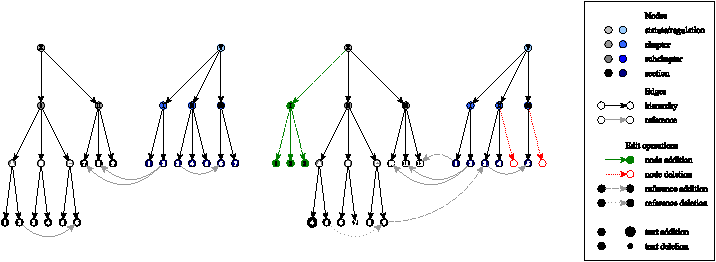
\includegraphics[width=\textwidth]{figure_2}
	\caption{Our legal network data model (adapted from \cite{katz2020}), illustrated for a dummy graph containing one statute and one regulation: initial configuration (left) and potential edit operations (right).}\label{fig:model}
\end{figure}

\vspace*{6pt}
\subsection{Data Model Instantiation}\label{subsec:data:instance}
To illustrate the power of the methodological framework laid out in Section~\ref{sec:methods} and produce the results presented in Section~\ref{sec:results}, we instantiate the data model described in Section~\ref{subsec:data:model} with the outputs of the legislative and executive branches of government at the national level in the United States and Germany, i.e., federal statutes and regulations, over the $22$~years from $1998$ to $2019$ (inclusive).
The rules contained in these sources are universally binding and directly enforceable through public authority (the combination of which distinguishes them from the other outputs listed in Table~\ref{tab:legal-system}).
In the United States and Germany, they are arranged into edited collections: the United States Code (USC) and the Code of Federal Regulations (CFR) in the United States, and the federal statutes and federal regulations (which have no special name) in Germany.
These collections are actively maintained to reflect the latest consolidated state of the law (though, in the United States, the consolidation may lag several years behind the actual law).
As such, they are a best-effort representation of all universally binding and directly enforceable rules at the federal level in their country at any point in time, commonly referred to as \emph{codified law}.

For the United States, we obtain the annual versions (reflecting the state of the codified law at the \emph{end} of the respective year) of the United States Code (USC) and the Code of Federal Regulations (CFR) from the United States Office of the Law Revision Council\footnote{\url{https://uscode.house.gov/download/annualhistoricalarchives/downloadxhtml.shtml}.} and the United States Government Publishing Office\footnote{\url{https://www.govinfo.gov/bulkdata/CFR}.}, respectively.
For Germany, we create a parallel set of annual snapshots for all federal statutes and regulations in effect at the \emph{end} of the year in question based on documents from Germany’s primary legal data provider, \emph{juris GmbH}.\footnote{
This differs from the approach taken in \cite{katz2020}, where the annual snapshots represented the law in effect at the \emph{beginning} of the year in question.
}
These data sources are the most complete presently available, 
but they may still be incomplete.
They also reflect choices made by and events affecting the agents in charge of their maintenance, e.g., varying rates and orders of updates, purposeful or unintentional omissions or modifications, and changes in the agents' composition (e.g., as a consequence of elections).

We perform several preprocessing steps on the raw input data, detailed in the Supplementary Information (\thesi), to extract the hierarchy, sequence, and reference structure contained in each collection.
The results are directed multigraphs, one per country and year, akin to those illustrated in Figure~\ref{fig:model}. 
These graphs contain all structural elements of the USC and the CFR (in the United States) or the federal statutes and regulations (in Germany) as nodes 
and all direct inclusion relationships (\emph{hierarchy}) and atomic references (\emph{reference}) as edges, where the references are resolved to the section level (\emph{sequence}).
Each graph represents the \emph{codified law} of a particular country in a particular year, containing documents of two \emph{document types} (statutes and regulations) at the federal level.

When modeling codified law as just described, we take a couple of design decisions that limit the scope of the results presented in Section~\ref{sec:results}. 
First, we focus on \emph{codified} law, i.e., \emph{law in books}, excluding other legal materials listed in Table~\ref{tab:legal-system}, especially those representing \emph{law in action} (in the sense of \cite{pound1910}),  
or even other representations of legislative materials such as the United States Statutes at Large or the German Federal Law Gazette (Bundesgesetzblatt).
These materials all merit investigation, and they need to be included in an all-encompassing assessment of the legal system. 
Our current work also serves as a preparatory step toward realizing this larger vision.

Second, we extract \emph{atomic} and \emph{explicit} references that follow a specified set of common patterns only, i.e., references including---in a typical format---a particular section (called ``Paragraph'' or ``Artikel'' in German law), a list of sections, or a range of sections.
With this procedure, we exclude \emph{container} references (e.g., references to an entire chapter of the USC), \emph{pinpoint} references (e.g., references to a codified Act of the United States Congress by its popular name), \emph{implicit} references (e.g., the use of a certain term implying its definition), and \emph{explicit} references following \emph{uncommon} patterns.
As sketched in Section~3.3 of the \thesi, there are plenty of such references, especially in the CFR, and including them would produce results different from those presented in Section~\ref{sec:results}.
However, the graph representation of such references is inherently ambiguous, 
and their extraction is inherently more challenging than the extraction of atomic citations.
Solving these problems falls outside the scope of this paper but presents an interesting opportunity for future work.

Third, we resolve the atomic references we extract to the level of sections, rather than the smallest referenced unit (which might be a subsection or even an item in an enumeration), thereby effectively discarding potentially valuable information.
Since for statutes and regulations, the section level corresponds to the documents' sequence level, this is consistent with our data model.
It also reflects a focus on the perspective of the user, who tends to navigate the law on the section level because it is the only level at which the individual German laws or their United States counterparts, the chapters of the USC and the CFR, are uniquely sequentially labeled. 
Finally, it ensures a certain degree of comparability because sections are the only structural elements in which text is (with very few exceptions) guaranteed to be contained (albeit the amount of text varies widely across sections).
Therefore, resolving references to the section level is reasonable for our purposes, but further research is needed on how the choice of the resolution level impacts the analysis of legal networks.
